\documentclass[letterpaper, 11pt]{article}
\usepackage[utf8]{inputenc}
\usepackage{amsmath}
\usepackage{wrapfig}
\usepackage{graphicx}
\usepackage[margin=0.7in,letterpaper]{geometry}
\usepackage{cite}
\usepackage[final]{hyperref}
\hypersetup{
	colorlinks=true,
	linkcolor=blue,
	citecolor=blue,
	filecolor=magenta,
	urlcolor=blue         
}
\usepackage{floatrow}
% Table float box with bottom caption, box width adjusted to content
\newfloatcommand{capbtabbox}{table}[][\FBwidth]

\begin{document}
\title{Juice Recommending System for Diseases}
\author{
	\texttt{Mohammed Saifuddin}\\
	\texttt{1640272 - 5CMS}
	\and
	\texttt{Mohammed Sameeruddin}\\
	\texttt{1640273 - 5CMS}
	\and
	\texttt{Purusharth Saxena}\\
	\texttt{1640207 - 5CMS}
}
\date{}
\maketitle
\subsubsection*{Introduction}
\paragraph{} This is a simple experimental project in machine learning, that implements the \texttt{TensorFlow API} to built a model for recommending juices to certain ubiquitous diseases like, cold, fever and sore-throat.
Recommending system essentially uses a filtering algorithm that brings all closely related units together from a dataset. There are certain practices which are dependent on the form of data, for our dataset, we implemented a neural network that \textit{classifies} diseases and then recommend the corresponding juice(s) for the cure of same.

Our dataset mainly comprises of 3 labels namely - \texttt{cold}, \texttt{fever}, \texttt{soarthroat}. Most of the juices do intersect at curing more than one disease, for example, Tomato juice cures both sore-throat and cold, but whereas Grapefruit juice just cures cold. Due to this intersection, we get 7 labels considering all the combinations. Below table shows labels of the dataset and respective numerical code.
\begin{center}
\setlength{\tabcolsep}{0.5em}
{\renewcommand{\arraystretch}{1}
\begin{tabular}{|p{5cm}||p{2cm}|}
\hline
\textbf{Label} & \textbf{Code}\\
\hline
\texttt{cold} & 0\\
\hline
\texttt{cold-fever} & 1\\
\hline
\texttt{cold-soarthroat} & 2\\
\hline
\texttt{cold-soarthroat-fever} & 3\\
\hline
\texttt{fever} & 4\\
\hline
\texttt{soarthroat} & 5\\
\hline
\texttt{soarthroat-fever} & 6\\
\hline
\end{tabular}
}
\end{center}

\begin{wrapfigure}{r}{0.35\textwidth}
\begin{center}
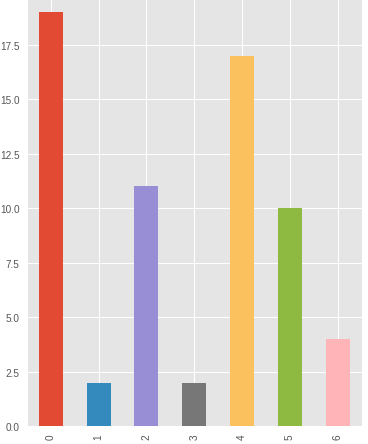
\includegraphics[width=58mm,scale=3]{sizez.png}
\caption{Sizes of each label}
\end{center}
\end{wrapfigure}

We have a visualization of the \texttt{sizes} for each label corresponding to their label names. In the graph, $x-$axis shows label-values that were coded and $y-$axis shows the respective sizes of each different label. With this bar graph we can comprehend that, \texttt{cold} and \texttt{fever} comprise a greater concentration in our data. Labels like \texttt{cold-fever} and \texttt{cold-soarthroat-fever} have the least number compared from the rest. Every column of the dataset is of numeric form except the \texttt{juice-names}. A machine learning model works smoothly only if the data is comprised of numbers, since we don't have numbers, we have \textit{integer-encode} that categorical columns. Integer encoding is a process of encoding text data into discrete numbers where in model does not face any impeding consequences during learning.

\subsubsection*{Building the Model}
\paragraph{} Before building a model, we have ensure that every \textit{feature} in the data must be in \textit{numeric-column}, this is because in real scenario not all datasets are numeric. In this dataset, \texttt{juice-names} columns are categorical, so we have to encode them into numbers. 

Once after encoding we constructed \textit{feature-columns} and an \textit{input pipeline function} called \texttt{my-input-fn} to channelize the data to the model as per the convenience of \texttt{TensorFlow} \texttt{Estimator} class.

\subsubsection*{Construction of Feature Columns}
\paragraph{} Feature columns play a radical role while channelizing the data, to the model. They enable transformation of raw-data into formats that \texttt{Estimators} API can use. \texttt{Estimators} is an eminent class of \texttt{TensorFlow} where all \textit{classification} and \textit{regression} algorithms are precoded. Data can be of cleaved into two aspects, \texttt{numeric} and \texttt{non-numeric}. To create a feature-column, we invoke \verb!tf.feature_column! module. We have two types of columns,
\begin{itemize}
\item \textit{Dense} - This column comprises of \verb!numeric_column!, \verb!indicator_column!, \verb!embedding_column!.
\item \textit{Categorical}: This has \verb!categorical_column_with_identity!, \verb!categorical_column_vocabulary_file!, \verb!categorical_column_vocabulary_list!, \verb!crossed_column!.
\end{itemize}
For our model, we had to only use \verb!tf.feature_column.numeric_column(features_in_the_data)!.

\subsubsection*{Input Function Pipeline}
\paragraph{} Input function is a pipeline function that takes examples from the data. Examples include both \texttt{features} and \texttt{labels}. With this function, we \texttt{slice} the data from tuple form, \verb!(feature, labels)! and then do \texttt{batching} and \texttt{shuffling} of the data.

\subsubsection*{Training the Model}
\paragraph{} In this aspect, we instantiate an \texttt{object} of \verb!tf.estimator.DNNClassifier()!. This is actually a deep neural network classifier to train the model with the data. This whole strand is so crucial. The object that is instantiated would be configured with an \texttt{optimizer} named \verb!tf.train.GradientDescentOptimizer()!. This takes a parameter \verb!learning_rate!, that can be any floating-point number. This parameter is referred as \textit{tuning-parameter}, which is tuned most of the time by a practitioner to revamp the performance. The object that was created, takes a parameter named, \verb!input_fn! which will be an implementation of pipeline function. Since \texttt{TensorFlow} is \texttt{Python} based, it is easy to create anonymous functions called \texttt{lambda}. We create a lambda function that invokes \verb!my_input_fn! and pass it to the \verb!input_fn! parameter.

With this we have a model, that has access to the data via, pipeline. Now we train it in a loop such that, the \textit{weights} are chosen that minimizes the \texttt{loss} function $L(x)$. Loss is defined as the difference between \texttt{true} function $f(x)$ and \texttt{hypothesis} function $h(x)$. Hypothesis function generalizes the true function. Gradually, the model reduces \texttt{loss} and learns to generalize the data-points.
\begin{figure}[h]
\begin{floatrow}
\capbtabbox{%
  \setlength{\tabcolsep}{0.5em}
{\renewcommand{\arraystretch}{1.2}
\begin{tabular}{|p{4cm}||p{2cm}|}
\hline
\texttt{Tuning-Parameters} & \texttt{Value}\\
\hline
\texttt{learning-rate} & $0.005$\\
\hline
\texttt{batch-size} & $3$\\
\hline
\texttt{steps} & $500$\\
\hline
\texttt{hidden-units} & $[8, 7, 6, 4]$\\
\hline
\end{tabular}
}
}{%
%   \caption{A table}%
}
\ffigbox{%
  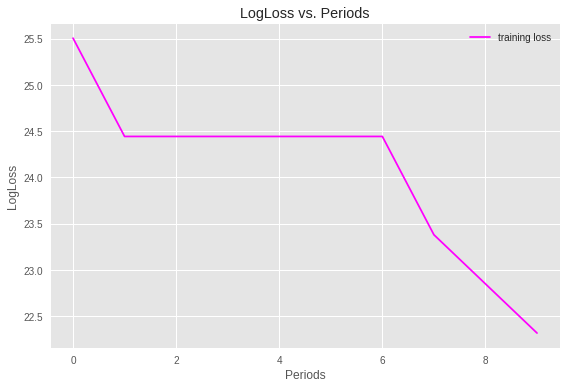
\includegraphics[width=70mm]{model_performance.png}
}{%
%   \caption{A figure}%
}
\end{floatrow}
\end{figure}
On the left, we have table of all tuning-parameters and their respective value. On the right we have \texttt{loss} gradually decreasing as the model started learning the data-points. Since we had only \texttt{65} units of data, the accuracy result that we obtained for this model was, \texttt{0.3538} or $35.3\%$.
\end{document}
